\section{Diagnostics techniques} \label{section:diagnostics-techniques}
Fault identification in the rotating machinery is a one-class or multi-class classification problem acting in a semi-supervised manner because labels for degraded conditions are scarce in practice. The automation goals in monitoring can be broadly categorized as anomaly detection and recognizing the momentary fault type.

The guiding principles for algorithm selection are simplicity in terms of their straightforward visual explanation for the production managers, and the ability to progressively improve the model on the streaming data to address peculiarities in individual machine constructions.

\subsection{Novelty detection}
Anomaly, novelty, or outlier detection determines whether a health status deviates considerably from the baseline profile. The expert can then step in and diagnose the machine after the notice. Anomaly is a rare observation different from the others, raising suspicion that it was created by unrelated behavior~\cite{aggarwal_outlier_2016}. The observations get assigned anomaly scores, and those over the threshold are novelties.

The measurements coming in the steaming fashion have to be processed in a single pass. The detection model must deal with the minimal admissible assumptions about the nature of the input events. The outliers are derived based on non-parametric statistical models, nearest-neighbor clustering, and isolation-based approaches~\cite{gervasi_anomaly_2020}.
\bigbreak

\textbf{DenStream} is a density-based algorithm adapted from DBSCAN to cluster streaming data of arbitrarily shaped groups. Samples it includes in the first step into coherent clusters are core data points in each other's neighborhoods. Core points have at least \emph{MinPts} ($\mu$) points in their neighborhood of radius \emph{Eps} ($\varepsilon$) units. Then non-core points in the proximity area of the core point are attached to the cluster containing it~\cite{aggarwal_data_2014}.

Quality of clustering results is evaluated by \emph{Silhouette score} in the range [-1; 1]. It demands points within clusters to have high cohesion and at the same time to have large separation from other clusters. The low score indicates a too small or too large number of clusters~\cite{rousseeuw_rousseeuw_1987}. 

\begin{figure}[ht]
    \centering
    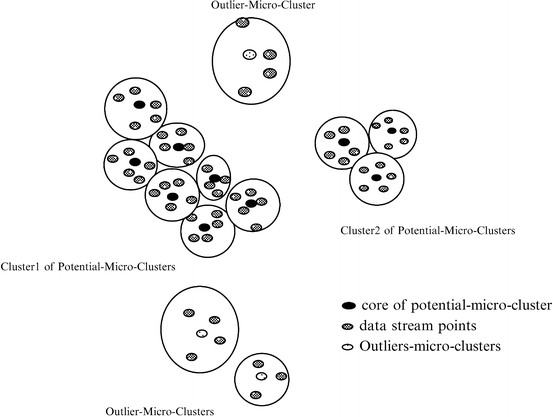
\includegraphics[width=0.8\textwidth]{assets/analysis/DenStream.png}
    \caption{DenStream~\cite{amini_density_2012}}
    \label{fig:denstream}
\end{figure}

In the online maintenance phase, DenStream summarizes the nearby observations into core \emph{micro-clusters} that can be potential micro-clusters or outlier \emph{micro-clusters} (Fig.~\ref{fig:denstream})~\cite{ghesmoune_state---art_2016}. The (outlier) \emph{o-micro-clusters} can grow into (potential) \emph{p-micro-clusters} when they encompass $\beta \mu$ points. The outliers are discounted after some time in accordance to the decay function: $f(t) = 2^{-\lambda t}$ or below the lower weight limit $\xi$. The on-demand offline stage runs DBSCAN over the approximate representation in micro-clusters to deliver final apportionment~\cite{cao_density-based_2006}.
\bigbreak

\textbf{Half-Space Tree} (HS-Tree) stands upon the concept of Isolation forest. It assumes that random splitting of each axis in the feature space will isolate outliers to their separate divisions sooner than non-deviant observations~\cite{gervasi_anomaly_2020,torres_automatic_2022}. This ensemble of trees is better suited for batch setting. HS-Tree stands out in adapting to changing streams because it is trained solely on normal data, requires constant memory, and is faster than density-based methods~\cite{tan_fast_2011}.

\begin{figure}[ht]
    \centering
    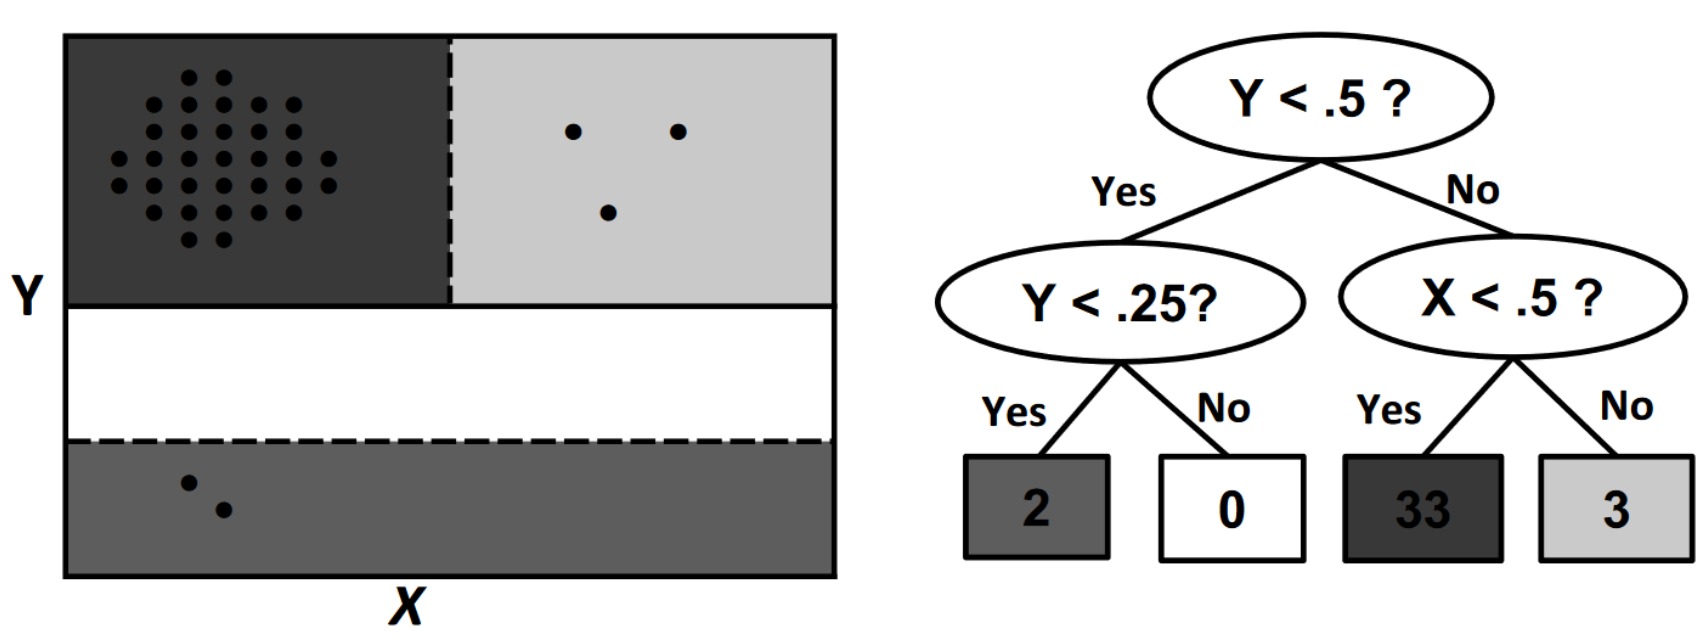
\includegraphics[width=0.8\textwidth]{assets/analysis/HS-Tree.png}
    \caption{Half-space tree~\cite{tan_fast_2011}}
\end{figure}

A full binary tree is built before the novelty detection begins by splitting tree nodes along the divisions in the randomly chosen perpendicular planes. The node stores its depth, value limits of the axis bisection (half-space), count of contained data points (mass) in two consecutive windows, and links to both child nodes~\cite{tan_fast_2011}. 

The anomaly profile in the latest window is always compared to the predecessor reference window. After the latest window is filled up, it replaces the reference window. It suffices to use a window size of 250 and an ensemble of 25 trees~\cite{tan_fast_2011}.

\subsection{Classification}
Accurate multi-class classification of machine fault causes according to the characteristics of known ones is a much more difficult task than novelty detection. Fault combinations have to be recorded and transformed into feature space. Interactions among fault root causes have to be considered. We are aware of rapid advances in knowledge transfer for deep neural networks~\cite{maurya_condition-based_2021}. So far, solutions seem not production-ready and hard to explain. Therefore, we opt to use a simpler model.

Performance of classification is estimated by several metrics on the validation set obtained using hold-out or cross-validation techniques. Frequently used quantities for classifier model evaluation include accuracy, precision, recall, f1 score, area under the ROC curve, and counts of hits and misses in a confusion matrix.
\bigbreak

\textbf{K-nearest neighbors} (kNN) assigns the data point to the class where the majority of $k$ closest instances belong (Fig.~\ref{fig:KNN}). It means it can work in a semi-supervised environment because it can infer labels just from knowing a few annotations. The major drawback of KNN is a preference for the majority class in imbalanced class-size datasets~\cite{shi_improving_2020}. The issue is mitigated with class weights or resampling classes by oversampling or undersampling. The KNN algorithm requires features to be normalized to assign the same importance to each predictor.

\begin{figure}[ht]
    \centering
    \begin{subfigure}[b]{0.49\textwidth}
        \includegraphics[width=\textwidth]{assets/analysis/KNN.png}
        \caption{KNN with k = 5}
        \label{fig:KNN}
    \end{subfigure}
    \hfill
    \begin{subfigure}[b]{0.49\textwidth}
        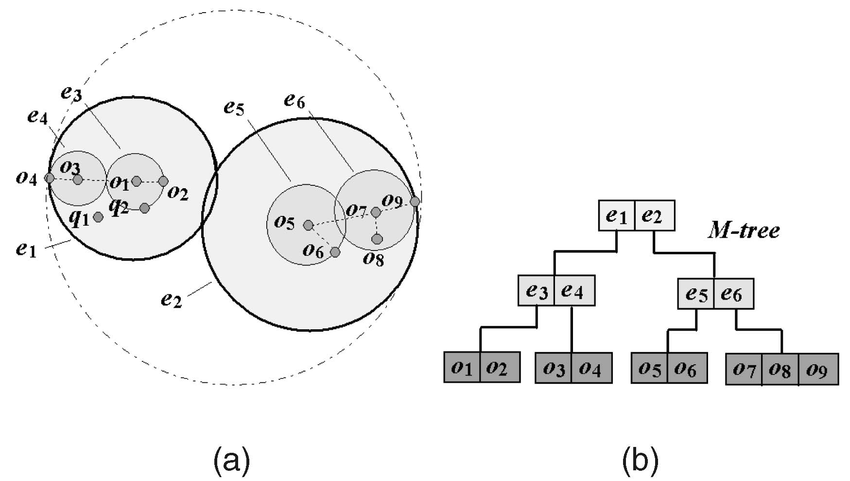
\includegraphics[width=\textwidth]{assets/analysis/M-tree.png}
        \caption{M-tree data structure}
        \label{fig:m-tree}
    \end{subfigure}
    \caption{Nearest neighbors classification algorithm~\cite{chen_skyline_2009}}
\end{figure}

The sense of distance between feature vectors $\mathbf{x}$, $\mathbf{y}$ have to be defined, so several metrics are available like \emph{Euclidian distance}, \emph{Mahalanobis distance}, \emph{Manhatann distance} etc. (Tab.~\ref{tab:KNN-distance})~\cite{sheng_review_2020, abu_alfeilat_effects_2019}. The optimal $k$ parameter is set by supervised learning according to the breaking point in the elbow curve that plots choices of $k$ against the error rate. The demanding neighborhood queries are sped up using spatial index in spatial databases that utilizes search tree such as kd-tree, R-tree, or M-tree.

\begin{table}[ht]
\centering
\renewcommand{\arraystretch}{2}
\begin{tabular}{|l|l|}
\hline
\textbf{Distance}     & \textbf{$d(\mathbf{x}, \mathbf{y})$}                                   \\ \hline
Manhatann distance	 & $ |x_i - y_i| $													   \\ \hline
Euclidian distance    & $ \sqrt{\sum_{i = 1}^{n}(x_i - y_i)^2} $                               \\ \hline
Mahalanobis distance  & $ (\mathbf{x} - \mathbf{y})^T C^{-1} (\mathbf{x} - \mathbf{y}) $       \\ \hline
\end{tabular}
\caption{Distance metrics for KNN}
\label{tab:KNN-distance}
\end{table}

The nearest-neighbor classifier has been successfully applied in machinery fault diagnostics. On the CWRU bearing dataset, the KNN with the accuracy of 96.2\% slightly outperformed SVM (95\%) on the combination of time and frequency-domain features, time-domain features - KNN 91.2\%, SVM 88.8\%, and frequency domain features - KNN (98.8\%), SVM (96.2\%)~\cite{jamil_feature-based_2021}. 

Comparison of KNN and KLDA on a feature set consisting of average, kurtosis, skewness, and standard deviation vectors in each domain has been conducted, achieving a data reduction rate of 95\%. Best accuracy was reached for PSD features with 99.13\% with KLDA and 96.64\% with KNN classifiers and Mahalanobis metric. The sampling frequency was set at 40 kHz~\cite{altaf_new_2022}. Despite KNN lagging in accuracy, we have to keep in mind annotations for faults were complete, and machine learning was not tested in a streaming context.

\subsection{Incremental learning}
Online or incremental machine learning operates on the streaming data, updating the model parameters with each new incoming event or in mini-batches. This approach finds its use in big data processing when the whole dataset is not available in advance or cannot be processed at once because of memory limitations. 

There are some additional obstacles to watch out for with incremental learning in comparison to batch learning~\cite{gepperth_incremental_2016}:

\begin{enumerate}
    \itemsep0pt

    \item \textbf{Concept drift} is defined as the change in data distribution function over time. The two types of concept drift are virtual and real. In virtual drift, changes occur only in the input distribution. Real drift means that the alteration comes to underlying functionality. Concept shift occurs with an abrupt change.

    \item \textbf{Stability-plasticity tradeoff} concerns the speed with which the model adapts to new information. The model can react quickly, making it less stable, or retain patterns for longer but become irresponsive to sudden shifts.

    \item \textbf{Model complexity} should be adjustable to ensure flexibility in unforeseen circumstances. Simpler models in the ensemble can also further increase prediction robustness. Resource limitation bound complexity from above.

    \item \textbf{Memory model} can store aggregates from seen observations and its typical examples or finite window of latest samples with forgetting factor.
\end{enumerate}


\textbf{Model benchmarking} in incremental learning is achieved by comparing models to their batch counterparts or using progressive validation~\cite{blum_beating_1999, halford_correct_2020}. It has been shown that incremental clustering algorithms have overall worse accuracy than batch versions~\cite{gepperth_incremental_2016}. In the validation process, precautions should be taken to prevent data leakage from future events into the past.

\begin{figure}[ht]
    \centering
    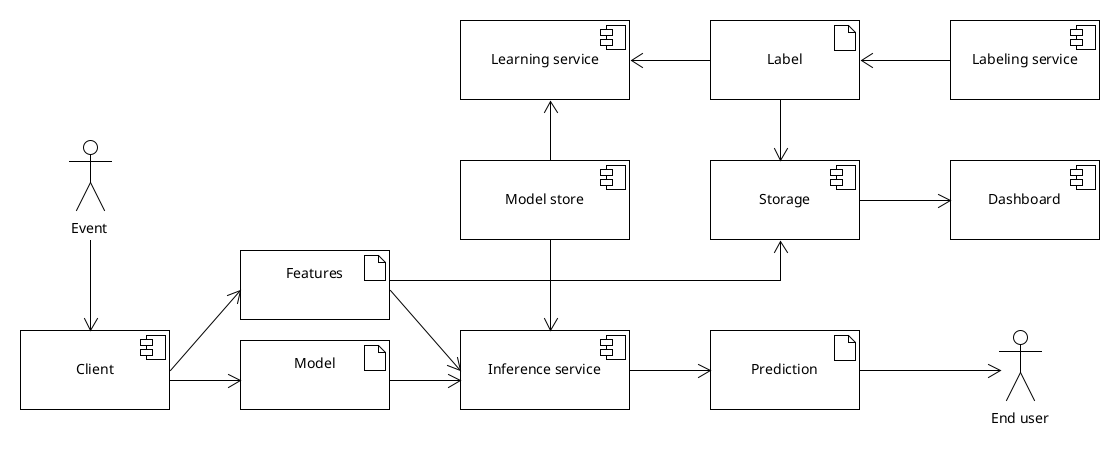
\includegraphics[width=\textwidth]{assets/analysis/incremental-learning.png}
    \caption{Incremental learning deployment architecture~\cite{gaia_online_2022}}
    \label{fig:online-learn-arch}
\end{figure} 

Deployment of an online machine learning model alongside supporting services is different from in established MLOps processes. Model store and Inference service components are supplemented with Labelling and Learning service~\cite{gaia_online_2022}. Their goal is to tune model parameters gradually as additional ground truth labels are provided. Labels can be provided later in a scheme called ``log and wait'', but data features are stored until such time.
  
